\documentclass[11pt,a4paper]{article}

\usepackage[utf8]{inputenc}
\usepackage[T1]{fontenc}
\usepackage{lmodern}
\usepackage{amsmath}
\usepackage{amssymb}
\usepackage{tikz}
\usetikzlibrary{arrows.meta,positioning}

\begin{document}

\section*{The Main Idea}

Our current system learns by \textbf{playing many games and adjusting a neural network}. GaP takes a different approach:
\textbf{AI coding assistants build a structured program, test it in simulation,
inspect failures, and improve the program.}

\noindent The difference is:

\begin{itemize}
    \item \textbf{Our PPO approach:} ``Keep practising until you learn what to do.''
    \item \textbf{GaP:} ``Build a plan from available skills, try it, understand what failed, and revise it.''
\end{itemize}

\subsection*{1. What the Paper Does}

The paper focuses on robots repeatedly doing the same kind of task, but with some variation. For example, packing groceries when the objects start in different positions. Instead of learning every movement from scratch, it provides a \textbf{library of skills}, such as finding an object, planning a movement, grasping, and checking whether an action succeeded. AI coding assistants connect these skills into a \textbf{graph}, essentially an executable flowchart:

\begin{center}

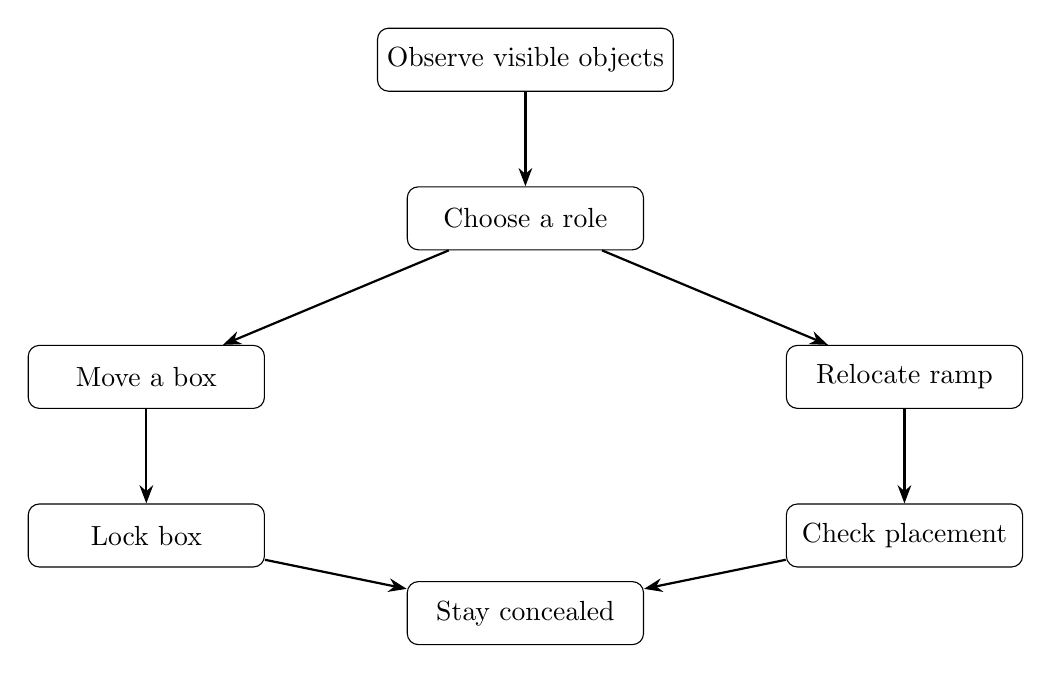
\begin{tikzpicture}[
    node distance=12mm and 18mm,
    box/.style={
        draw,
        rounded corners,
        align=center,
        minimum width=30mm,
        minimum height=8mm
    },
    arrow/.style={
        -{Stealth},
        thick
    }
]

\node[box] (observe) {Observe visible objects};

\node[box, below=of observe] (role) {Choose a role};

\node[box, below left=of role] (move) {Move a box};

\node[box, below right=of role] (ramp) {Relocate ramp};

\node[box, below=of move] (lock) {Lock box};

\node[box, below=of ramp] (check) {Check placement};

\node[box, below=of role, yshift=-30mm] (concealed) {Stay concealed};

\draw[arrow] (observe) -- (role);

\draw[arrow] (role) -- (move);
\draw[arrow] (role) -- (ramp);

\draw[arrow] (move) -- (lock);
\draw[arrow] (ramp) -- (check);

\draw[arrow] (lock) -- (concealed);
\draw[arrow] (check) -- (concealed);

\end{tikzpicture}

\end{center}

The graph contains both actions and decisions. It is the robot's policy: the thing that determines what it does.

\subsection*{2. How It Improves}

The paper's learning loop is:

\begin{enumerate}
    \item Generate an initial graph from the task description and available skills.
    \item Test it on multiple variations of the task.
    \item Record what happened and where failures occurred.
    \item Have the coding assistants change the graph, its parameters, or individual skills.
    \item Repeat.
\end{enumerate}


\subsection*{3. How We Could Apply It to our Scenario}

We can keep our \textbf{MuJoCo quadrant environment, game rules, actions, and rewards}. We would add a separate GaP-style system around it.

A first hider graph looks like:

\begin{center}

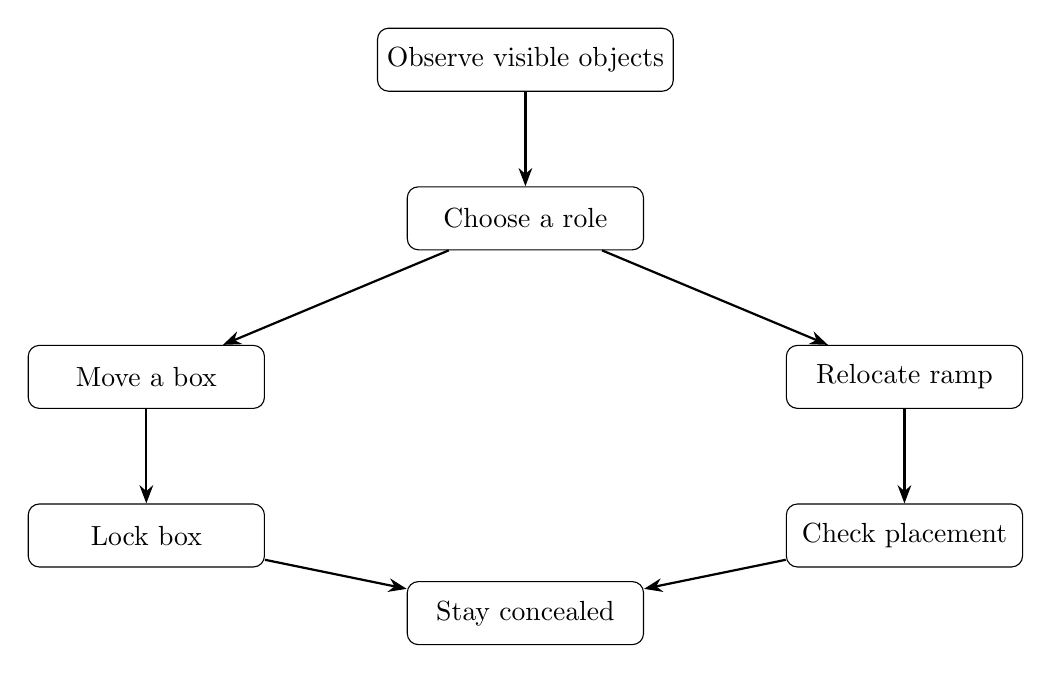
\begin{tikzpicture}[
    node distance=12mm and 18mm,
    box/.style={
        draw,
        rounded corners,
        align=center,
        minimum width=30mm,
        minimum height=8mm
    },
    arrow/.style={
        -{Stealth},
        thick
    }
]

\node[box] (observe) {Observe visible objects};

\node[box, below=of observe] (role) {Choose a role};

\node[box, below left=of role] (move) {Move a box};

\node[box, below right=of role] (ramp) {Relocate ramp};

\node[box, below=of move] (lock) {Lock box};

\node[box, below=of ramp] (check) {Check placement};

\node[box, below=of role, yshift=-30mm] (concealed) {Stay concealed};

\draw[arrow] (observe) -- (role);

\draw[arrow] (role) -- (move);
\draw[arrow] (role) -- (ramp);

\draw[arrow] (move) -- (lock);
\draw[arrow] (ramp) -- (check);

\draw[arrow] (lock) -- (concealed);
\draw[arrow] (check) -- (concealed);

\end{tikzpicture}

\end{center}


\subsection*{3. First Experiment}

Start with \textbf{GaP-style hiders against a fixed collection of our existing seeker checkpoints}. 

Compare the initial graph, the improved graph, and our existing PPO hiders on held-out episode seeds. Measure win rate, performance against different seekers, simulation episodes, wall-clock time, and LLM cost.


\end{document}